\chapter{Magnolia 5.0 AdminCentral Module Architecture}
\label{architecture}

The biggest part of the Magnolia 5.0 project is the design and development of
the AdminCentral module - a replacement for the former \emph{AdminInterface}
module. Improved user interface is one of the major targets for AdminCentral
module.

However, the role of AdminCentral is supposed to go far beyond the UI
shell. It is the point of intersection between most of the other modules, a
framework that allows to create complex abstractions on top of their
functionality and provide an easy way to set up communication between them.
In order to fulfill the aforementioned design requirements for extensibility and
mobile platforms support - it was decided to emulate the environment of an
operating system for CMS administration. The resemblence is of course supposed
to be metaphorical, design-wise. The main idea is to have an environment with a
chrome and applications that run inside of it. Such a pattern allows for
creating the additional functionality by merely developing another application.
In order to maintain the common look and feel for all types of platforms the
mobile-like way of UI arrangement was chosen: Single Document Interface (SDI)
with a dashboard and the applications that consume the whole viewport one at a
time.

the AdminCentral is to provide a framework for the applications: both
initial and additional apps must be equally easy to develop, the amount of the
boilerpalte code has to be minimal and the least amount of programming skills
should be required.

The role of \emph{Vaadin} framework in the \emph{AdminCentral} is to make it
possible to achive the compromise between the rich UI and the development
clearness and simplicity.
With Vaadin it is possible to design the entire application development system
completely on the server-side: the user interface can be generated directly form
the configuration templates kept in the storage (JCR) and the powerful
client-server communication mechanism can be used for emulating the navigation
 (based on the browser-fragments).
\section{Architecture Overview}

\begin{figure}[H] \centering 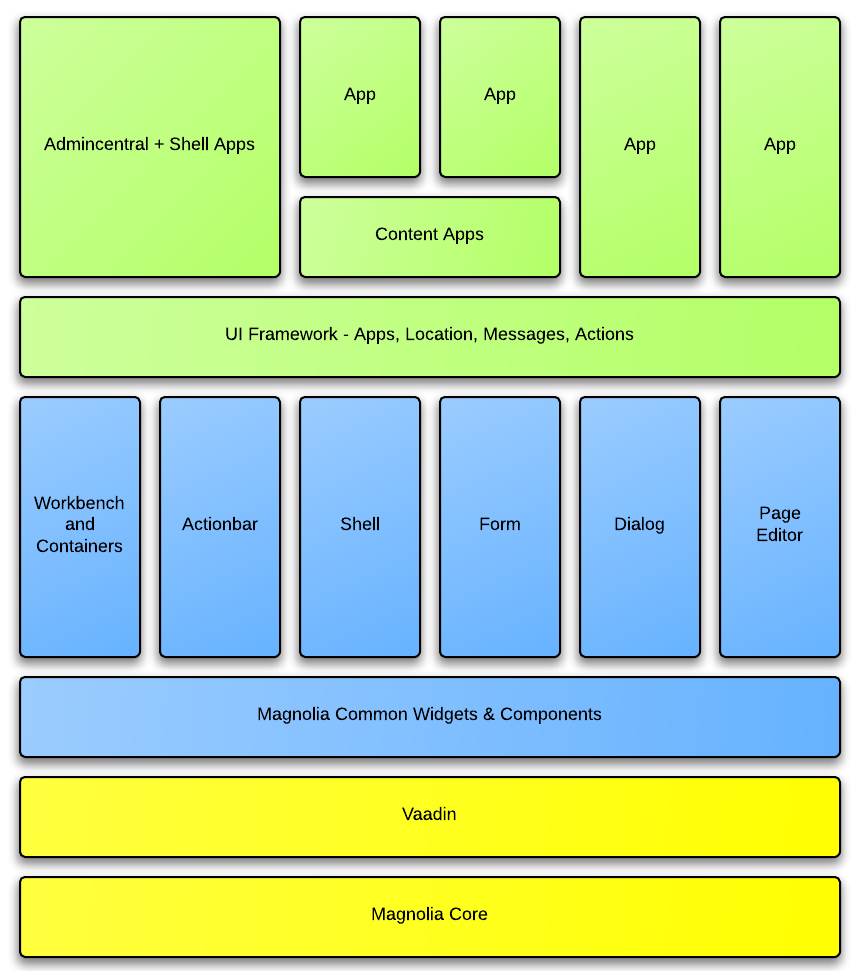
\includegraphics[width=\textwidth]{architecture_layers.png}
	\caption{High-level architecture overview}
	\label{fig:architecture_overview}
\end{figure}

Firgure ~\ref{fig:architecture_overview} displays the structure of the project
architecture. The main goal of a such architecture design is to provide a set of loosely
coupled components and interfaces. The block structure means that every block is
a separate Magnolia CMS module which encapsulates a logical part of the system.
The firgure ~\ref{fig:architecture_overview} also describes the dependency
hierarchy of the project: the parts of the system can only depend on the blocks
that belong to the layer that resides below in the diagram. This means that most
low-level tiers of the architecture are core Magnolia API and plain Vaadin
components and interfaces, whereas the top-level parts are apps - parts of the
system actually visible to an end-user. Apps can re-use any API and frameworks
present in the system. Let us briefly discuss the features of all the layes of
the architecture.

\subsection{Magnolia Core API and Vaadin} 
  The main two frameworks used in the system
  provide a low-level foundation of Magnolia AdminCentral module. Magnolia Core
  API enables interfaces and utilities for accessing JCR, dependency injection
  functionality, tools for localization etc. Vaadin serves as a platform for the
  Magnolia AdminCentral web-application and abstract building blocks
  (Components) for moe specific parts of teh system.
\subsection{Magnolia Common Widgets and Components} 
  This layer of the system aggregates the essential re-usable components built on top of the core
  frameworks. Such components include, for instance, the page editor - the
  What-You-See-Is-What-You-Get (WYSIWYG) utility for modifying the website
  pages. Common Components layer also includes the data management structures
  such as JCRContainer.
\subsection{UIFramework} 
  UIFramework layer provides the foundation for the apps,
  such as base classes and interfaces, action-execution mechanisms and message
  exchange infrastructure. UIFramework also contains the fundamental
  communication framework for the entire AdminCentral web application, which is
  called Location Framework.
\subsection{AdminCentral and apps}
  Finally, the top-most architecture layer is reserved for apps and AdminCentral
  web application. An app represents a logically and functionally consistent
  unit that allows for conducting certain operations on the contnet and/or the
  essentail workflow utilities.

In the current chapter we will mostly discuss the concept of the UIFramework in
detail. The importance of UIFramewor cannot be overestimated because it is a connection
point between the core API's and comonents and the apps. We will pay additional
attention to the app-framework as well. The following chapter
(\ref{implementation}) will highlight the implementation details of the most
crucial components from the common widgets layer.

\section{Technology Stack Roles Distribution} 
Before starting to explore the parts of Manolia 5.0 architecture in details and
analyzing how they solve the problems stated in \ref{thesis_problems} it is
important to clarify the communication relationships between the frameworks used
in the project. We also need to define which framework acts on the server-side
and which - on the client-side. Let us consider the high-level outline of
project's structure displayed on the figure \ref{fig:architecture}:

\begin{figure}[H] \centering 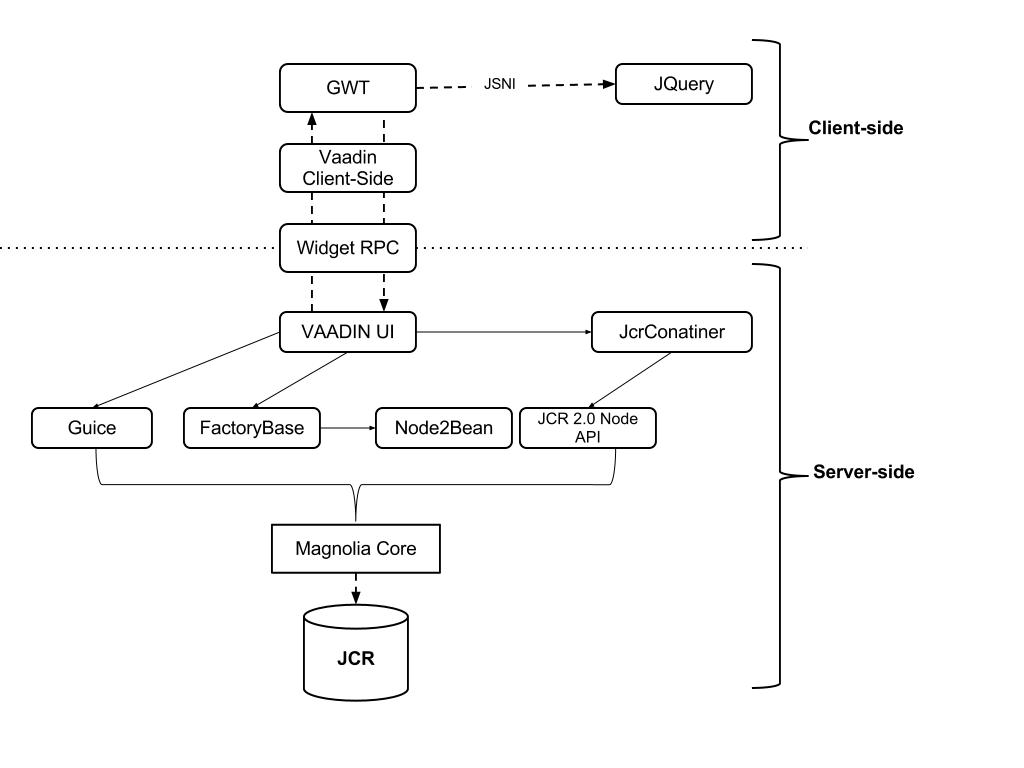
\includegraphics[width=\textwidth]{architecture.jpg}
	\caption{Magnolia CMS 5.0 Architecture}
	\label{fig:architecture}
\end{figure}

\paragraph{JCR} repository is at the lowest level of the hierarchy and stores
not only the content and templates but also all the configuration for the
system:
\begin{itemize}
  \item The structure of the user interface building blocks.
  \item Registries of the functionality units used within the system and the way
  they are accessible for the user.
  \item Binding between the action definitions that can be performed on the
  nodes and their implementation.
\end{itemize}

\paragraph{Magnolia Core} API's provide the low-level communication mechanism of
interaction with JCR and implementation for the various patterns that can be
re-used in the project. The most important parts of it include for instance the
API for querying the JCR and Node2Bean that allows for projecting the nodes to
Java Beans transparently to the developer. Another crucial framework provided by
the Magnolia Core is the Dependency Injection (DI) functionality based on Google Guice
\cite{google_guice}. The main strength of this framework is that allows to
define the mapping between the interface and the implementation of the
components right in a module descriptor - all the other configuration is done
internally and the developer does not have to take care of it, it is usually even
not necessary to know what DI mechanism actually provides the fucntionality.

\paragraph{Vaadin} layer is based on top of JCR and Magnolia Core API's. It
plays a role of the foundation for the AdminCentral web application. Vaadin
generates all the components and views of the system based on the information
provided by the configuraion. The datasources for the components are normally
provided in a form of the \texttt{JcrContainer} which is an implementation of
the Vaadin's \texttt{Conatiner} interface based on top of the JCR Node API.
Vaadin resides in the top level of the server-side architecture. 

\paragraph{Vaadin} interacts with the client-side by means of its core
communication mechanism (UIDL, see \ref{chapter_tech_stack}) and by means of an
additional API provided by the WidgetRPC add-on. The latter is used in order to
improve the clearness and simplicity of communication. UIDL
communication allows for passing the numerous variables between the client and
the server, resulting in rather complex code structures that analyse the
incoming changes.

Contrary to the plain UIDL, WidgetRPC allows for building the communication
interfaces and mutually call the methods between the component's counterpart,
making the conversation between them more fine-grained and roust.

Vaadin client-side part is responsible for handling both ways if the
communication and also controls the resuting UI presentation.

\paragraph{Finally, GWT} is responsible to produce the views on top the commands
and instructions that are coming through the Vaadin's client-side engine.
Whereas the simpliest vaadin applicaton does not require the programmer to engage
GWT into the development (core Vaadin's widgetset could be enough) Magnolia 5.0
project requires a variety of the custom components to be built so that the
resulting interface gets all the necessary components without significant
overhead caused by adopting the ones from the core. In order to increase the
performance and to provide some complex UI effects the JQuery library was
incorporated into the project's client-side ramework. The access to JQuery can
be done directly from GWT.

\section{Location Framework}
We will start a detailed discussion about the UIFramework with an in-depth look
into the structure of the AdminCentral web application and its backbone - the
\emph{Location Framework}.

As it was discussed in the beginning of the chapter AdminCentral web application
is based on Vaadin framework. According to chapter \ref{chapter_tech_stack}
Vaadin applications work on top of Java Servlet API and any logic that is
executed within application is triggered by user input within the web browser.
An application is responsible for loading, displaying and closing the proper
views on a screen in response on the various events. Typically Vaadin
application would create, attach or detach components, set up the references
between them and update the states of components.

We have stated in chapter \ref{thesis_problems} that one of the most crucial
goals of the project is to provide an extensible and highly-customizable user
interface allowing for adding and removing the functional components on demand.
This requirement implies that AdminCentral web application must obtain an
abstact framework for the state management. An obvious solution would be to
provide mappings between possible URL's and the views. Such mappings should be
easilly customizable and the views should be possible to be pre-created as well
as generated on the fly (e.g. - based on the parameters of the query). All these
statements bring us to the navigation management framework called \emph{Location
Framework}.

Navigation handling is one of the most common problems that Rich Internet
Applications (RIA) developers face. For instance - dealing with poor support of
the browsers' history. The source of the problem is the fact that the frameworks
like GWT usually provide capabilities for building the single-paged applications
with an only one highly dynamic page that generates HTML-views according to
UI-logic. In such situations teh browser is not responsible for tracking the
navigation. For instance if a user presses the "back" button he will most likely
navigate away from the application, which is usually not the desired behavior.
However, this problem is possible to handle by means of a framework. GWT, for
instance, provides the API for the interaction with a web-browser history based
on fragments.
Fragment is a part of a URL after the hash sign (\#). Changing a URL-fragment
does not trigger a browser refresh, so a framework can provide the track of an
application internal navigation history by manually pushing the items into
browser history \cite{gwt_historian}.  Let us consider an example:
\url{http://www.example.com/example_app#view1}

In this example everything before the hash sign \texttt{(\#)} is the example-app
URL and the \texttt{view1} is the identifier of some application UI state. If a
user navigates to this URL in a browser GWT will fire an internal event and the
application client-side logic will determine which user interface parts to
display.

However, URL fragment is just a tool that could be used for navigation.The main
problem is how to effectively map the multiple views that a complex Rich
Internet Application might provide to the corresponding URL fragments. It also
should be possible to serialize the state of the views in the fragment and many
others.
For native GWT applications the framework team has provided a rather flexible
and useful sub-framework called Activities and Places framework
\cite{activities_places}.

Activities and Places is a design pattern for structuring the navigation in a
user interface. The parts of an application are its activities and they can be
reached by activating their respective place. For web applications a place is
derived from the browser URL allowing a section of the application to be
bookmarked. As the user interacts with the application the browser URL changes
in response to place changes.

Activities and Places framework is widely used by the GWT community. However,
for a server-side oriented application like Magnolia 5.0 AdminCentral it would
be impossible to use it for navigation, as the client-side is rather thin. As a
consequence it was decided by the development team to port the framework to the
server-side and adopt it for Vaadin-based applications. The resulting concept is
called the Location framework. The name location was chosen to substitute the
term place because it reflects the web nature of the application better: the
current URL of a RIA or a site is obtained by calling \texttt{window.location}
in JavaScript.  Let us consider the Locations framework in details.

\subsection{Location}

\begin{figure}[H] \centering 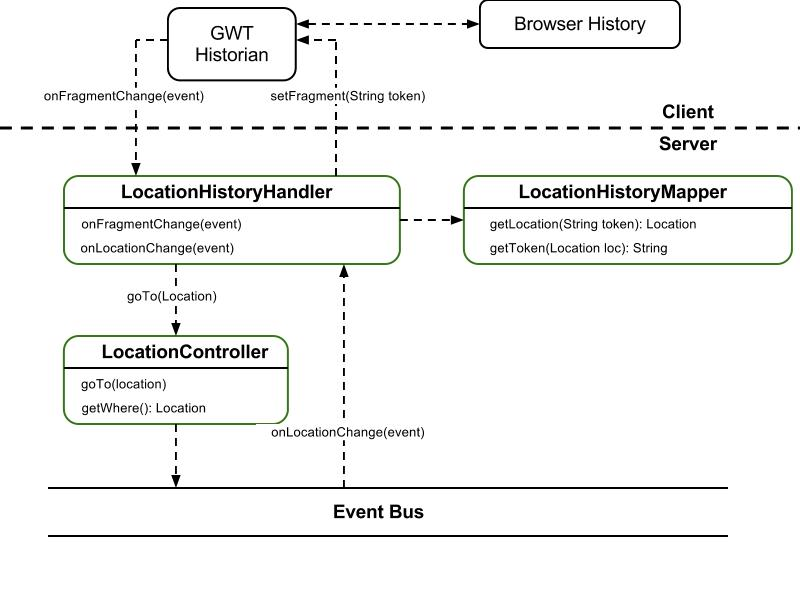
\includegraphics[width=\textwidth]{location_arch.jpg}
	\caption{Location framework pt.1}
	\label{fig:location_arch}
\end{figure}

\subsubsection{Location} 
Location is a data transfer interface between the server-side and
the browser history. It is capable of deserializing a fragment string into a 
Plain Old Java Object (POJO). That POJO in turn can serialize itself into a
valid URL fragment string.

\subsubsection{Event Bus}
 The backbone of the Location framework is the EventBus
(\emph{TODO Consider EventBus pattern appendix}). One global event bus acts as a communication
channel between other parts of the framework. For instance, it gets notified of
the fragment change from the client-side and triggers the user interface
change sequence. On the other hand, when a UI update is initiated on the
server-side due to some user input and an application navigates to a new
location, an event bus propagates the new location to all the interested
parties. The location is eventually transformed into the fragment and ends up on
the client-side in the browser history.

\subsubsection{Location Controller} \texttt{LocationController} is a singleton
(/*consider appendix*/) object that handles navigation between locations and keeps
current location. \texttt{LocationController} is tightly
connected with the event bus:
the latter accepts the listeners and transmits the events fired by the
controller. In order to perform navigation to a different location through the
\texttt{LocationController} one has to simply call the following:

\begin{lstlisting}
	locationContoller.goTo(location);
\end{lstlisting}

Such a call changes and controller's current location and causes it to emit a
LocationChangeEvent on the event bus. A good example of a
\texttt{LocationChangeEvent} handler would be some kind of a UI manager that
would find and/or construct the appropriate view depending on a location.

\subsubsection{LocationHistoryHandler and LocationHistoryMapper} 
Another entity that handles the \texttt{LocationChangeEvents} is
\texttt{LocationHistoryHandler}.
It is the connection point between the framework and the web browser. It is
capable of converting the location into a string (URL fragment) and vice-versa -
obtaining a location by a fragment. However, \texttt{LocationHistoryHandler}
does not accomplish these tasks on its own rather than that - delegating the
implementations of search and conversion to a \texttt{LocationHistoryMapper}.
\texttt{LocationHistoryMapper} as it is stated in its title maps the unique
history fragments to corresponding locations in a bi-directional way.


\subsection{Activities and ActivityManagers}
\begin{figure}[H] \centering 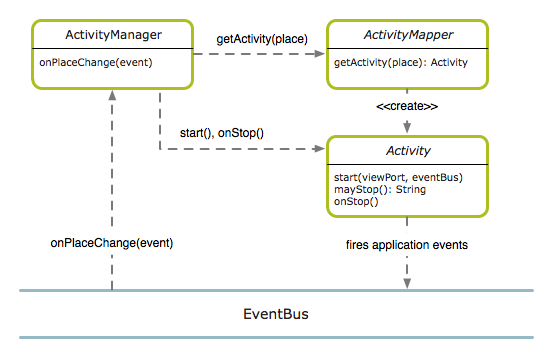
\includegraphics[width=\textwidth]{activities.png}
	\caption{Location framework pt.2}
	\label{fig:location_arch}
\end{figure}

\subsubsection{Activity}
\texttt{Activity} is the concept of the original framework from Google Web
Toolkit. Its main purpose is similar to the role of the Presenter in
Model-View-Presenter pattern which will be discussed later in the current
chapter (see \ref{MVP}). Provided with a state snapshot stored in a location and
a viewport for rendering an \texttt{Activity} is able to handle state,
initialize, update, load and unload the \texttt{View}\cite{activities_places}.
\texttt{Activity} is also able to notify the other objects (e.g. a different
\texttt{Activity}) about its internal events through the framework's
\texttt{EventBus}.
 
\subsubsection{ActivityManager and ActivityMapper}
\texttt{ActivityManager} and \texttt{ActivityMapper} classes purpose is to
resolve an
\texttt{Activity} that corresponds to an incoming \texttt{Location}.
\texttt{ActivityManager} subscribes to an \texttt{EventBus} and awaits for new
\texttt{Locations}.An \texttt{ActivityMapper} is used as a registry that mapps 
an \texttt{Activity} to a \texttt{Location}.

In Locations framework the role of the Activities is played by the
\emph{Apps} and the job of \texttt{ActivityManager}
and \texttt{ActivityMapper} is done by an \texttt{AppController} (see \ref{section_apps}).


 
\section{Model-View-Presenter}
\label{MVP}
As we have discussed before - \emph{Location Framework} provides an abstract and
convenient functionality to map the application logic to the changes triggered
by means of the URL fragments changes. We mentioned Model-View-Presenter (MVP)
pattern in that discussion as a connector between the URL fragment and the
actual \texttt{View}.

However, this is not the only use case of this pattern within the project: it
appears to be useful when separation between user interface and its presentation
logic is required. Let us explore the concept of the Model-View-Presenter
pattern and the ways of its adoption in Magnolia 5.0 application.

Model-View-Presenter (MVP) pattern is one of the cornerstone patterns of
Magnolia 5.0 user interface. A lot like the classic Model-View-Controller (MVC)
pattern MVP aims for the separation of user interface implementation from the
presentation logic.
\begin{figure}[H] \centering 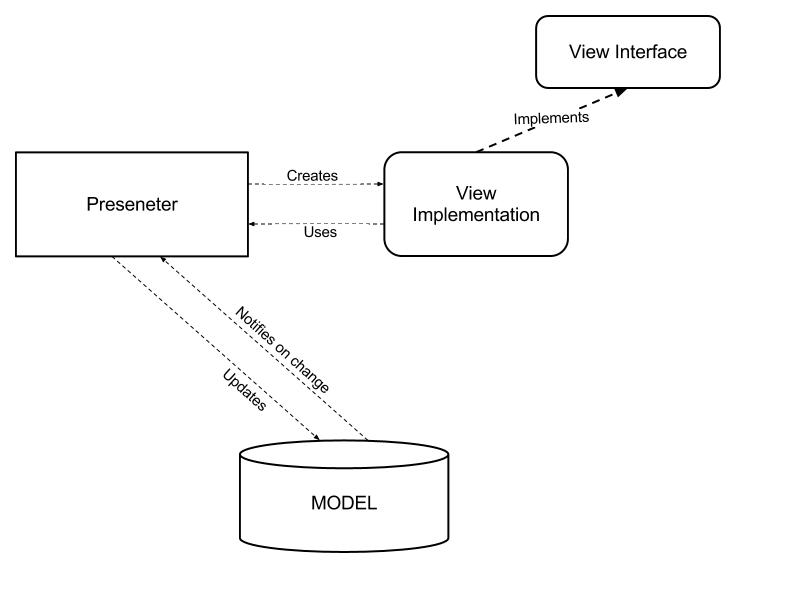
\includegraphics[width=\textwidth,
height=\textheight, keepaspectratio]{mvp.jpg}
	\caption{Model-View-Presenter}
	\label{fig:mvp}
\end{figure}
Advantages that Model-View-Presenter pattern offers are:
\begin{itemize}
  \item Clear design with completely separated handling of UI events form the actual handlers logic.
  \item Possibility to re-use interfaces of the views and presenters interfaces for different implementations.
  \item Separated test for the UI and for logic. 
\end{itemize}

\subsection{Presenter} Presenter exposes an interface that contains methods for all the actions that could be triggered in a view
like search, filtering, update etc. As an action is invoked by the view the presenter executes the necessary operation,
accessing model if needed. After that the presenter updates the view accordingly. Presenter is also responsible for
reaction on the changes of model not triggered by the current view.

\subsection{View} The view is logically clear composition of a set of user interface components that displays and/or gathers data
from the user. The view interface exposes all the methods that a presenter might need to assemble and steer it (e.g.
access to the parts of the view, getters/setters for some fields etc.). Ideally the view is not supposed to be bound to
any UI technology completely concealing its implementation from the presenter, so the presenter tells the view what to
do, whereas it is up to the view to decide how to do it. In case of Magnolia 5.0, however, we will break this rule and
for almost all the cases oblige the view to expose itself as a Vaadin component (because Vaadin is the only UI
technology used on the server-side).

\subsection{Model} Model is a data source used by a presenter. In Magnolia
CMS model is obviously a JCR repository. However, direct
access to JCR would be quite cumbersome and inefficient, so the actual communication with presenters in Magnolia 5.0
happens through the Vaadin data binding layer - a special JCR container, which will be discussed in the following chapter.

As it was already mentioned, MVP resembles Model-View-Controller pattern. However, in classic MVC the controller has to 
listen to both the View and the Model. This means, for instance, that the button click and text change handlers are registered
there. In MVP, on the other hand, the presenter only implmenets a set of certain functions that are invoked by the view.
Thus, MVP provides better decoupling between the view and the presentation. 

Besides already mentioned specialties of MVP use in Magnolia 5.0 (like a constraint to Vaadin) it is worth mentioning
that the main responsibilities are distributed differently than usual. Normally it is the job of the view to initialize
the presenter whereas in Magnolia 5.0 it is vice versa and the presenter creates the view. This difference is caused by
how the user interface is persisted in the back-end: JCR configuration repository contains only the information how to
build the UI which is a description of the presenter. Later when the user navigates to some specific view a pre-created
presenter instantiates the actual UI component.
\section{Configuration in Magnolia CMS}
By means of the \emph{Location Framework} and \emph{MVP} pattern which were
described before we have defined a foundation for an abstract loosely coupled
system which is capable loading, rendering and disposing some components.
Adding a new functionality in such a system would only require to
implement its logic and to add the proper mapping, so the system would load the
component on demand. However, the end developer should not be required to change
the source files or mapping configuration manually. Instead there should be an
interface by means of which the developer would interact with the system and
alter its state. In the current section we will analyze the approach of a
high-level definition mechanism used in Magnolia 5.0.

Configuration mechanism is an essential feature of many software products. It
enhances the flexibility and extensibility in the sense that the person without
deep knowledge of the system internals can alter its behavior, re-arrange and
customize its parts. 

Magnolia CMS is also configurable by means of XML. Each module has an XML
descriptor containing all the properties needed for its description. An example
of a configurable component could be a registry of the forms with fields which
would be represented with a set of XML nodes with properties and sub-nodes for
fields types, captions, default values, validators etc. 

Most of Magnolia CMS configuration files are kept within \emph{config}
workspace. Displaying this workspace in a form of editable tree would allow the
user to modify the components visually in real time as long as the system
instantly reacts on those changes.
There are several techniques in Magnolia CMS that are used for applying the
configuration. The main two concepts are \emph{observation} and \emph{Node2Bean}.

\paragraph{Observation} is a feature of JCR that allows for subscribing to the
changes in a workspace. Observing applications can monitor and react on those
changes whenever the persistent operation is made in JCR. This feature has found
various ways of applications in Magnolia CMS. For instance, one of the most
important ways is the foundation for the factory-based [TODO: consider factory
appendix] structures: some sort of bindings are stored in a workspace in a form
of the registry which is later used in the factory to produce the actual objects.

\paragraph{Node2Bean} is used to convert the JCR nodes into the Java objects. 

By means of Java Reflection (introspection mechanism) Node2Bean binds the the
fields of a Java Bean to the corresponding configuration properties (if such are
available) through the bean's "setter" and "adder" methods. Node2Bean can
support all possible data types:
\begin{itemize}
  \item Simple data types like \texttt{String, int, long, float, double, boolean}.
  \item Collections with String values or other data types by specifying a class property.
  \item Maps with keys and values as Strings or other data types by specifying a class property.
  \item Complex classes can be mapped with Node2Bean by means of the sub-nodes
  which follow the same rules and restrictions.
\end{itemize}

Let us consider an example of using Node2Bean:

\begin{figure}[H]
	\centering
	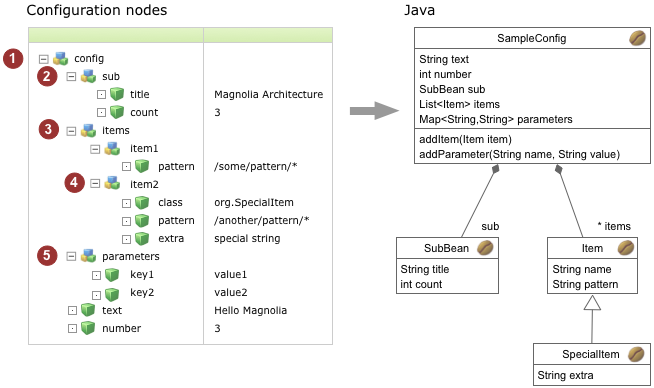
\includegraphics[width=\textwidth]{node_to_bean.png}
	\caption{Node2Bean mapping example}
	\label{fig:node2bean}
\end{figure}

Numbered items:

\begin{itemize}
  \item config: Entry point of the transformation. In the module descriptor
  \texttt{SampleConfig} class is used. Set text and number properties.
  \item sub: Sub bean. The class is determined using reflection if it is not
  explicitly defined.
  \item items: Collection. The corresponding add method is used to determine the
  class and populate the collection if existing.
  \item item2: Special item with its own class and additional properties.
  \item parameters: Collection of key-value pairs.
\end{itemize}

\section{It Is All About Apps}
\label{section_apps}
Magnolia 5.0 introduces applications of simply \emph{apps} to content
management. An \emph{app} stands for the configurable, pluggable unit which
encapsulates some certain functionality that typically operates over the data
stored in the JCR repository.
Magnolia 5.0 comes with a special framework for app management. This framework
is integrated with Magnolia CMS configuration mechanism which provides the
data required to start an app and Location Framework which triggers various
events causing app load, unload and navigation. 
There are two types of apps in Magnolia 5.0 - besides of apps of a regular type
(e.g for page editing or workspace browsing) there are special administrative so
called \emph{shell-apps}.

\subsection{Apps} An app is \emph{a tool with a very narrowly focused interface
enabling CMS users to work on one set of closely related tasks or one specific
set of data. An app does not necessarily work on a single, physical data set
(e.g. the pages of a site), but may cover multiple physical data sets required
to solve the task it covers.} \cite{maui_apps}. It is worth mentioning that in
case of Magnolia 5.0 app is not an application per se but rather a concept of a
user interface metaphor.

\subsection{App Framework}
The \emph{App Framework} is a name for Magnolia 5 functionality that manages
apps. This involves interaction with Magnolia CMS configuration mechanism:
handling the app registry and reacting on changes in app configuration.
It also controls an app life-cycle events such as starting, displaying, and
stopping an app \cite{wiki_app_framework}. Finally, the App Framework keeps the contexts of loaded apps,
maintaining their state and order.

\subsubsection{App Configuration}
The primary configuation of the apps is done by means of the
\texttt{AppDescriptor} class. \texttt{AppDescriptor} is a simple Plain Old Java
Object (POJO) that holds the meta information like the app name, label and its
icon. A descriptor also carries the name of a class that actually implements the
app and a list of \emph{sub-app} descriptors. A \emph{sub-app} is an entity that
implements the part of an app functionality. The \texttt{SubAppDescriptor} class
resembles an analogous for the app except for the fact the sub-app is a terminal
structure, so it has no child descriptors. 

In order to provide a higher level configuration mechanism for apps it is
possible to describe App descriptors in JCR inside the \emph{config} workspace.
As the Magnolia CMS web application starts up the descriptors are mapped to Java
classes by means of the Node2Bean mechanism:

\begin{figure}[H] \centering 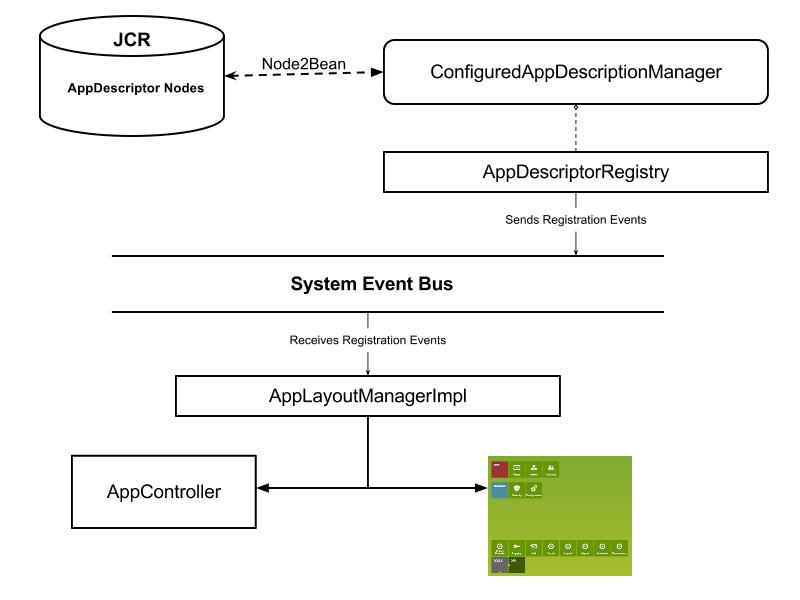
\includegraphics[width=\textwidth]{app_configuration.jpg}
	\caption{Registration of Apps.}
	\label{fig:app_registry}
\end{figure}

An instance of the \texttt{ConfiguredAppDescriptorManager} obsreves the changes 
in \emph{config} workspace and translates the JCR nodes that stand for the app descriptors to 
the objects of type \texttt{AppDescriptor}.

The scanned descriptors are then placed into the \texttt{AppDescriptorRegistry}
which fires the corresponding events for registration, deregistration or update.
The main receiver of such kind of events is an implementor of the so called
\texttt{AppLayoutManager} class. The purpose of this class is to maintain the
order of registered apps and to display them properly in the user interface (in
\emph{AppLauncher} shell-app) and to make them available to the navigation
system (the app controllers).

\begin{figure}[H] \centering 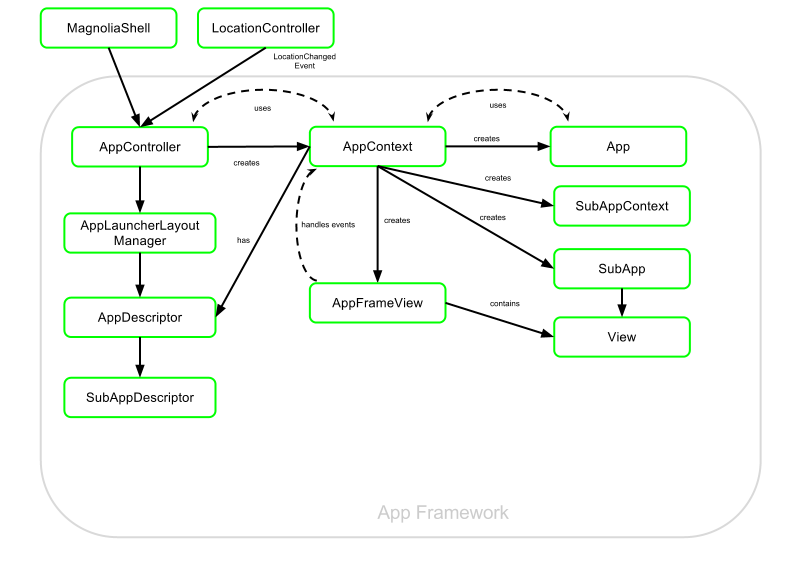
\includegraphics[width=\textwidth]{app_controller.png}
	\caption{App Context Management}
	\label{fig:app_context}
\end{figure}

\subsubsection{App Controllers and App Context.} The cornerstones of the \emph{App Framework} are the two
controller objects: \texttt{AppController} and \texttt{ShellAppController}.
These two objects play a similar role as \texttt{ActivityManager} in the original 
Places framework of GWT and apps are the analogues of \texttt{Activity}.
Controllers are subscribed to \texttt{LocationChangeEvent}'s. Based on the
incoming \texttt{Location}s either of two controllers retreives an app context.
\texttt{AppContext} is the class that holds the state of an app that is up and
running.

\begin{lstlisting}
public interface AppContext 
{
    void openSubApp(Location location);
    void start(Location location);
    void stop();
    void onLocationUpdate(Location newLocation);
    
    AppDescriptor getAppDescriptor();
    App getApp();
    
    View getView();
    String getName();    
    String mayStop();
}
\end{lstlisting}

As it is visible from the aforementioned fragment of an interface -
\texttt{AppContext} is able to react on \texttt{Location} changes. The
implementor of an interfaces typicaly conducts it by starting the app or one of
its sub-apps. An \texttt{AppContext} allocates the view component that would
host a new app (typically it is a tab-sheet component). It is also responsible
for providing all the neccessary paramteres to a newly created app or sub-app,
like dependency injector, reference to the context itself (so that the app could
indirectly communicate to the \emph{App Framework}) and location.

As the \texttt{start(\ldots)} method is called an \texttt{AppContext}
instantiates the sub-class of the \texttt{App} interface declared in the app
descriptor.

The \texttt{App} sub-class is basically a \emph{presenter} for a concrete app
implementation. We will cover the examples of app development in the
implementation chapter.

\subsection{Shell Apps.} There are three and only three shell apps that are
responsible for administration functions of the system. Those are called
\emph{AppLauncher}, \emph{Pulse} and \emph{Favorites}. \emph{AppLauncher} is a
dashboard with app icons allowing for starting apps and navigating between them.
\emph{Pulse} is an area that contains and receives the notifications and messages for a
user. Finally, \emph{Favorites} aggregates links and bookmarks allowing for better
customization of the system.
\section{Magnolia Shell}
As long as the architecture splits the functionality units into apps it is
logical to assume that there must be an environment that would host and
manipulate those apps. In Magnolia 5.0 such an environment is called
MagnoliaShell.

Magnolia Shell is the main part of Magnolia 5.0 user interface foundation.
Primarily the component is responsible for displaying and laying-out the apps
and for performing transitions between them, which makes it a core UI container
of the project.
MagnoliaShell is also highly important part of the architecture due to its
integration with other parts of the system.
 

\begin{figure}[H] \centering 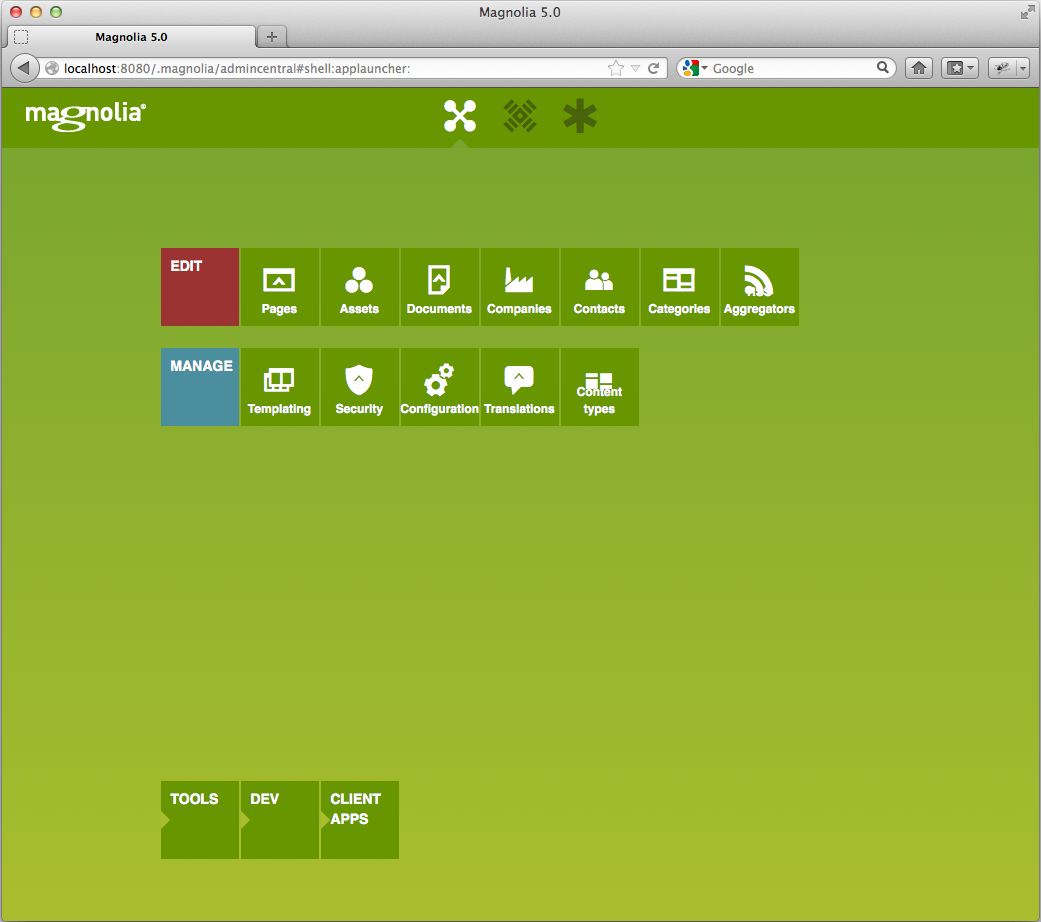
\includegraphics[width=\textwidth]{magnolia_shell.png}
	\caption{Magnolia Shell}
	\label{fig:m_shell}
\end{figure}

From the user interface point of view MagnoliaShell conceptually resembles the
browser viewport \cite{mshell_wiki}.
Actually, it contains two viewports (\texttt{ ShellViewport}): one for the apps
and one - for the shell apps.
 The \emph{ application framework } utilizes the viewports as containers in
 \texttt{AppController} and \texttt{ShellAppController} implementation.

\emph{Locations framework} is also connected with MagnoliaShell. The latter acts
as a buffer between client and server sides in fragment handling process. The
client-side implementation of MagnoliaShell subscribes to GWT's History API
events, based on a fragment it resolves which type of an app it has to launch
and instructs the server accordingly. On the server-side the
\texttt{LocationHistoryHandler} de-serializes the received fragment into a
\texttt{Location} instance which is handled by either \texttt{AppController} or
\texttt{ShellAppController}: based on the location parameters the correct
sub-app is launched. The other way around - an app is able to initiate a
navigation event (e.g. when switching between two app due to some server side
logic), at the end simply forcing the browser to update its fragment silently
(without sending an event to subscribers).

\section{Actions}
http://wiki.magnolia-cms.com/display/DEV/Actions+API+and+configuration
http://wiki.magnolia-cms.com/display/MAGNOLIA5/UI+-+Actions
http://wiki.magnolia-cms.com/display/UX/The+action+bar+screens

\section{Dependency injection}
\input{include/architecture/di.tex}

\pagebreak